\documentclass[border=4pt]{standalone}
\usepackage{tikz}
\usepackage{pgfplots}
\pgfplotsset{compat=1.18}
\usetikzlibrary{shapes.geometric,arrows.meta,positioning,fit,calc,decorations.pathreplacing}
\usepackage{xcolor}
\definecolor{bestcol}{HTML}{1565C0}
\definecolor{freegreen}{HTML}{2E7D32}
\definecolor{learnblue}{HTML}{1565C0}
\definecolor{fusred}{HTML}{C62828}
\newcommand{\best}[1]{{\color{bestcol}\textbf{#1}}}
\begin{document}
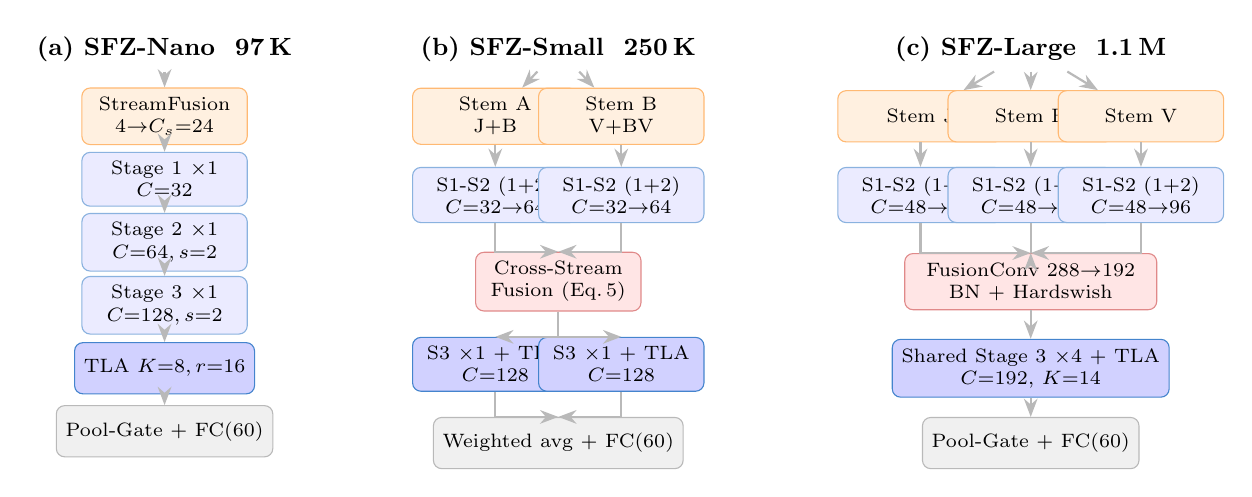
\begin{tikzpicture}[
  every node/.style={font=\scriptsize},
  blk/.style ={draw, rounded corners=3pt, minimum width=2.1cm,
               minimum height=0.65cm, align=center,
               fill=blue!8, draw=learnblue!50},
  stem/.style={blk, fill=orange!12, draw=orange!55},
  fus/.style ={blk, fill=red!10,    draw=fusred!55},
  cls/.style ={blk, fill=gray!12,   draw=gray!55},
  tlabox/.style={blk, fill=blue!18, draw=learnblue!80},
  tit/.style={font=\small\bfseries},
  arr/.style={-Stealth, thick, draw=gray!55}
]

%% ─── (a) Nano ──────────────────────────────────────────────────────────────
\node[tit] (na_t) at (0, 0) {(a) SFZ-Nano\ \ 97\,K};
\node[stem]   (na_sf)  at (0,-0.85)  {StreamFusion\\$4{\to}C_s{=}24$};
\node[blk]    (na_s1)  at (0,-1.65)  {Stage 1 $\times$1\\$C{=}32$};
\node[blk]    (na_s2)  at (0,-2.45)  {Stage 2 $\times$1\\$C{=}64,s{=}2$};
\node[blk]    (na_s3)  at (0,-3.25)  {Stage 3 $\times$1\\$C{=}128,s{=}2$};
\node[tlabox] (na_tla) at (0,-4.05)  {TLA $K{=}8, r{=}16$};
\node[cls]    (na_cl)  at (0,-4.85)  {Pool-Gate + FC(60)};

\foreach \a/\b in {na_t/na_sf, na_sf/na_s1, na_s1/na_s2,
                   na_s2/na_s3, na_s3/na_tla, na_tla/na_cl}
  \draw[arr] (\a)--(\b);

%% ─── (b) Small ─────────────────────────────────────────────────────────────
\node[tit] (sm_t) at (5.0, 0) {(b) SFZ-Small\ \ 250\,K};

\node[stem] (sm_sfA) at (4.2,-0.85) {Stem A\\J+B};
\node[stem] (sm_sfB) at (5.8,-0.85) {Stem B\\V+BV};
\node[blk]  (sm_12a) at (4.2,-1.85) {S1-S2 $(1{+}2)$\\$C{=}32{\to}64$};
\node[blk]  (sm_12b) at (5.8,-1.85) {S1-S2 $(1{+}2)$\\$C{=}32{\to}64$};
\node[fus]  (sm_csf) at (5.0,-2.95) {Cross-Stream\\Fusion (Eq.\,5)};
\node[tlabox](sm_s3a) at (4.2,-4.00){S3 $\times$1 + TLA\\$C{=}128$};
\node[tlabox](sm_s3b) at (5.8,-4.00){S3 $\times$1 + TLA\\$C{=}128$};
\node[cls]  (sm_cl)  at (5.0,-5.00) {Weighted avg + FC(60)};

\draw[arr] (sm_t)--(sm_sfA);
\draw[arr] (sm_t)--(sm_sfB);
\draw[arr] (sm_sfA)--(sm_12a);
\draw[arr] (sm_sfB)--(sm_12b);
\draw[arr] (sm_12a.south) -- (sm_12a.south |- sm_csf.north) -- (sm_csf.north);
\draw[arr] (sm_12b.south) -- (sm_12b.south |- sm_csf.north) -- (sm_csf.north);
\draw[arr] (sm_csf.south) -- (sm_csf.south |- sm_s3a.north) -- (sm_s3a.north);
\draw[arr] (sm_csf.south) -- (sm_csf.south |- sm_s3b.north) -- (sm_s3b.north);
\draw[arr] (sm_s3a.south) -- (sm_s3a.south |- sm_cl.north) -- (sm_cl.north);
\draw[arr] (sm_s3b.south) -- (sm_s3b.south |- sm_cl.north) -- (sm_cl.north);

%% ─── (c) Large ─────────────────────────────────────────────────────────────
\node[tit] (lg_t) at (11.0, 0) {(c) SFZ-Large\ \ 1.1\,M};

\node[stem] (lg_sfJ) at ( 9.6,-0.85) {Stem J};
\node[stem] (lg_sfB) at (11.0,-0.85) {Stem B};
\node[stem] (lg_sfV) at (12.4,-0.85) {Stem V};
\node[blk]  (lg_12J) at ( 9.6,-1.85) {S1-S2 $(1{+}2)$\\$C{=}48{\to}96$};
\node[blk]  (lg_12B) at (11.0,-1.85) {S1-S2 $(1{+}2)$\\$C{=}48{\to}96$};
\node[blk]  (lg_12V) at (12.4,-1.85) {S1-S2 $(1{+}2)$\\$C{=}48{\to}96$};
\node[fus,minimum width=3.2cm] (lg_fc)
                     at (11.0,-2.95) {FusionConv $288{\to}192$\\BN + Hardswish};
\node[tlabox,minimum width=3.0cm]
             (lg_s3) at (11.0,-4.05) {Shared Stage 3 $\times$4 + TLA\\$C{=}192,\,K{=}14$};
\node[cls]   (lg_cl) at (11.0,-5.00) {Pool-Gate + FC(60)};

\draw[arr] (lg_t)--(lg_sfJ);
\draw[arr] (lg_t)--(lg_sfB);
\draw[arr] (lg_t)--(lg_sfV);
\draw[arr] (lg_sfJ)--(lg_12J);
\draw[arr] (lg_sfB)--(lg_12B);
\draw[arr] (lg_sfV)--(lg_12V);
\draw[arr] (lg_12J.south) -- (lg_12J.south |- lg_fc.north) -- (lg_fc.north);
\draw[arr] (lg_12B.south) -- (lg_12B.south |- lg_fc.north) -- (lg_fc.north);
\draw[arr] (lg_12V.south) -- (lg_12V.south |- lg_fc.north) -- (lg_fc.north);
\draw[arr] (lg_fc)--(lg_s3);
\draw[arr] (lg_s3)--(lg_cl);

\end{tikzpicture}
\end{document}
